\section{Experimental}

%Characterize the system, give all details that matter. Describe how the experimental procedure went.

% CAS codes Hinzufügen?

\subsection{Chemicals}
The following experiments were conducted using sodium carbonate, anhydrous, (\qty{105.99}{\gram\per\mole}), from \texttt{Sigma Aldrich}, puriss., (\qty{99.5}{\percent}, calc. to the dried substance), and potassium carbonate (\qty{138.2}{\gram\per\mole}), from \texttt{Sigma Aldrich}, (\qty{99}{\percent}). All chemicals were used forgoing any further purification.

Additionally, a premixed $\approx$ \qty{0.1}{\M} calcium chloride solution was used. Its origin and purity are unknown to the authors.

\subsection{Procedure}
A total of 5 experiments were prepared and carried out as follows:

\begin{figure}[H]
    \centering
    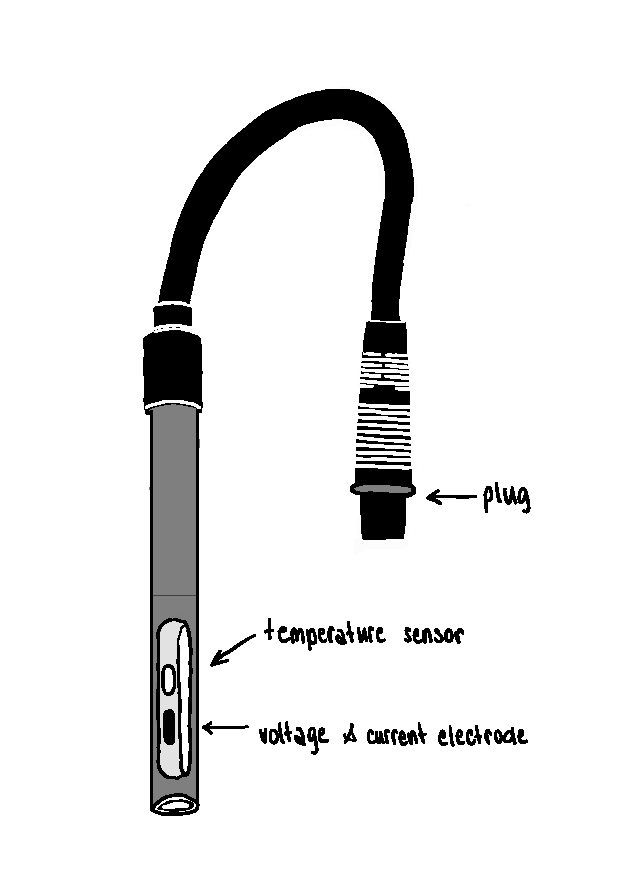
\includegraphics[width=.5\textwidth]{figures/Conductometer.pdf}
    \caption{The \texttt{KNICK SE 204} measuring cell can measure values ranging from \qty{1.00}{\micro\siemens\per\centi\meter} - \qty{500}{\milli\siemens\per\centi\meter} and has a cell constant of approximately \qty[per-mode=reciprocal]{0.5}{\per\centi\meter}}
    \label{fig:sketch_cond}
\end{figure}






\subsubsection{Specific conductivity of water}

First, the specific conductivity $\kappa$ of differently treated water samples was measured using a \texttt{KNICK 703} conductometer with a \texttt{KNICK SE 204} 4-pole measuring cell (Fig. \ref{fig:sketch_cond}). Three samples were prepared for deionised water, ultrapure deionised and degassed water (from a \texttt{HUBER and CO. AG} TKA-GenPure), and tap water each and the respective conductivity measured immediately after preparation (especially for deionised and degassed water) to ensure that the results would not be falsified by any compounds formed through contact with the surrounding air. 


%\newpage

\begin{figure}[H]
    \centering
    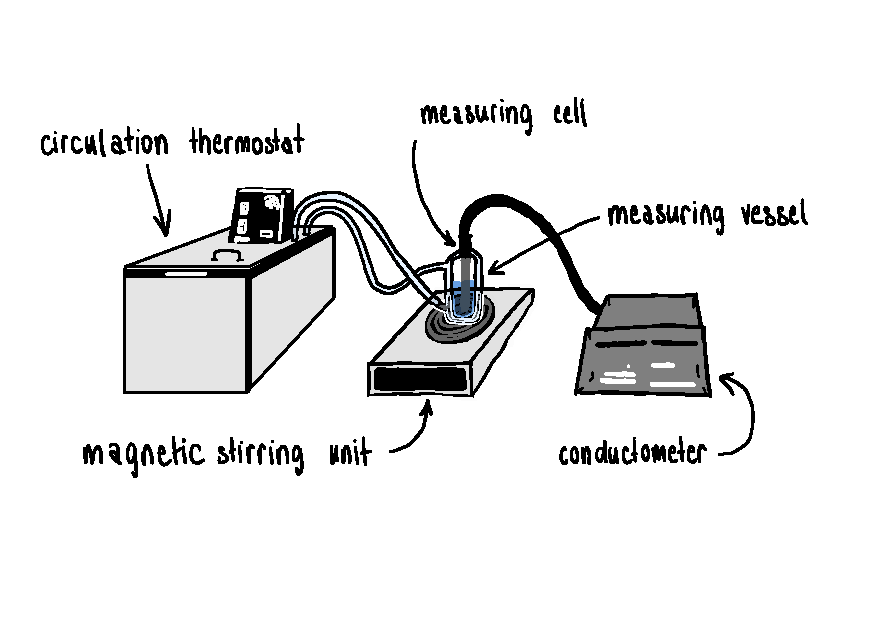
\includegraphics[width=.5\textwidth]{figures/Conductometer_bigpicture.pdf}
    \caption{The entire setup for conductivity measurements, including the \texttt{LAUDA MT} circulation thermostat, the \texttt{KNICK SE 204} measuring cell and the \texttt{KNICK Conductometer 703}.}
    \label{fig:sketch_cond_2}
\end{figure}

\subsubsection{Correlation between temperature and conductivity}

For the next experiment, the specific conductivity $\kappa$ of a 0.1 M potassium carbonate solution was measured at steadily decreasing temperature. 
The solution was prepared by weighing \qty[round-precision=5]{1.3895}{\gram} of sodium carbonate in a \qty{100}{\milli\liter} volumetric flask using a \texttt{METTLER TOLEDO AG204 Delta Range} analytical balance and filling the flask to its mark with deionized water. 
The sample was transferred to the measuring vessel (Fig. \ref{fig:sketch_cond_2}) and heated to \qty{50}{\celsius} by means of a \texttt{LAUDA MT} circulation thermostat. The specific conductivity at \qty{50}{\celsius} was noted in the lab journal and subsequently the heat supply to the circulation thermostat cut off, simultaneously activating the water cooler to bring the temperature of the sample to a gradual, steady decline. 
Finally, $\kappa$ of potassium carbonate in a 0.1 M aqueous solution was noted down for temperatures between \qty{50} {\celsius} and \qty{25}{\celsius} in steps of \qty{1}{\celsius}.



\subsubsection{Molar conductivity of different electrolytes} 

Next, the molar conductivity $\Lambda$ of \qty{0.01}{\M} solutions of potassium carbonate and sodium carbonate was calculated using values obtained from measurements of $\kappa$ at constant temperature for both solutions. 
The potassium carbonate solution was prepared by taking \qty{50}{\milli\liter} of the solution used in the previous experiment and diluting it with water at a 1:10 ratio. 
The sodium carbonate solution was prepared similarly to the potassium carbonate solution in the previous experiment, by weighing \qty{0.5298}{\gram} of sodium carbonate in a \qty{100}{\milli\liter} volumetric flask and filling it to its mark.
Samples of both solutions were transferred to the measuring vessel separately and their respective conductivity noted down after brief stirring. This was repeated twice more for each solution.

\subsubsection{Concentration dependency of conductivity and limiting molar conductivity}

For the next experiment, the specific conductivity $\kappa$ of a \qty{0.01}{\M} sodium carbonate solution was measured at constant temperature and increasing concentration $c$. 
First, a \qty{10}{\milli\liter} burette was rinsed out and then filled with the same solution as in the previous experiment. Then the measuring vessel was filled with \qty{100}{\milli\liter} of deionized water (measured by means of a volumetric flask) and its intrinsic conductivity documented. Finally, the sodium carbonate solution was added in steps of \qty{0.5}{\milli\liter} and the conductivity of the resulting solution noted down after each increase until a total of \qty{10}{\milli\liter} had been added. 

\subsubsection{Conductometric titration}

For the last experiment, a potassium carbonate solution of unknown concentration was provided by the laboratory assistant, of which exactly \qty{100}{\milli\liter} were transferred to the measuring vessel via volumetric flask. A \texttt{METROHM 775} dosimat was filled with the titer, for which a pre-prepared \qty[round-precision=5]{0.09997}{\M} calcium chloride solution was provided. The titer was released into the potassium carbonate solution via "Go" button in approximately \qty{0.5}{\milli\liter} steps, noting down the exact volume that was added and the corresponding concentration after every increment. A total of \qty{20}{\milli\liters} calcium chloride was added to the solution. 





% ===============================================================
% ==================OLD STUFF====================================
% ===============================================================

\iffalse{


\subsubsection{measuring conductivity of different solutions}

measuring conductivity of differnt types of water, versch elektrolytlösungen, versch. salze in wasser,  eines salzes bei 

wie funktioniert conductometer (KNICK 703 und 4-Pol-Messzelle KNICK SE 204 
integrierter NTC Temperatursensoror

kann gleichzeitig 

0.09997 M cacl2







The identity and purity of acetone and n-hexane were verified by determining their respective \textit{refractive index} and \textit{density}. 






\textit{Refractive index} measurements were done via digital refractometer \texttt{ATAGO RX-5000} operating at standard wavelength of \qty{589.0}{\nano\meter} (D-line) and with samples maintained at a constant \qty{20.00 \pm 0.02}{\celsius} by a \texttt{LAUDA E100} circulation thermostat (attached to the refractometer). After ensuring the glass surface of the sample block was dry, a small amount of liquid was applied – just enough to cover the circular surface – and once equilibration was reached as indicated by the temperature display, measurements could be initiated.

\textit{Density} was determined in two different ways.

First, by \textit{method A}, filling a \qty{25.00 \pm 0.04}{\milli\liter} volumetric flask (insert marke) with either liquid and measuring its mass using a \texttt{METTLER-TOLEDO AG204 Delta Range} analytical balance, the accuracy range of which is stated as \qty{0.1}{\milli\gram} by the manufacturer.

And secondly, by \textit{method B}, using an \texttt{ANTON PAAR DMA 48} density gauge (Fig. \ref{fig:sketch_rho}), where the respective sample was carefully inserted via plastic syringe and – after visual confirmation that there were no air bubbles inside the u-shaped glass tube – run at setting \mintinline{R}{F505}. Between measurements of different samples, the tube was rinsed with deionized water and dried by inducing airflow.





The boiling temperatures of acetone and n-hexane were measured at different pressure settings. 

For this purpose, a two necked flask containing the sample and about 10-15 boiling stones and filled to approximately half its capacity was attached to a pre-prepared setup (Fig.\ref{fig:sketch_setup}), omitting grinding grease due to the risk of contaminating the sample and comparatively low significance of a tight seal in this experiment.

Only after ensuring that all openings were closed, the \texttt{BÜCHI VAC V-503} vacuum pump, dimroth condensation cooler and \texttt{WINKLER WHLG2} laboratory heating mantle with a \texttt{WL10} heating controller were turned on. It is important to note that forgoing the former here and starting the cooler before sealing the system would allow water vapor from the air to condense inside the cooler and likely lead to falsified results. 

While maintaining a low heat supply via the controllable heating mantle, pressure within the system was steadily decreased under close surveillance through evacuation by means of a \texttt{BÜCHI I-100} vacuum controller and a ventilation valve until about \qty{150}{\milli\bar} and \qty{100}{\milli\bar} were reached for acetone and n-hexane respectively and the liquid was simultaneously boiling inside the flask and dripping steadily from the cooler. For acetone we could not observe any dripping at first, yet the liquid seemed to be boiling and the temperature was quickly decreasing to under \qty{10}{\celsius}. We concluded that the vapor currently forming would be at a lower temperature than the liquid in the dimroth cooler, causing it to escape into the separator instead of condensing. As such we increased our heat supply and not long after, equilibrium returned to the system and steady dripping could be observed. 

The temperature measured by the \texttt{GREISINGER GMH 3210} digital temperature gauge (with a resolution of \qty{0.1}{\kelvin}) was marked down with its corresponding vapor pressure and the pressure was incremented in \qtyrange{25}{50}{\mbar} steps until reaching \qty{900}{\mbar}, waiting for the temperature to level out after each increase and recording respective values. This was repeated at decreasing pressure, generating two sets of values for each sample.

%\newpage






The evaporation cooling effect of acetone, n-hexane and methanol (reference sample) were visualized and recorded by measuring the surface temperature of an ultra-sensitive heat sensor at \qty{0.25}{\second} intervals during the evaporation of a predefined volume of liquid sample applied to the sensor.

The setup, a \texttt{TREVAC}-apparatus (transient evaporation cooling) as can be seen in Fig. \ref{fig:sketch_trevac}, self-developed by the \texttt{PCL} at \texttt{ETH Zürich}, relies on a \texttt{LAUDA Ecoline 103} thermostat to keep the aluminium block with the \texttt{NATIONAL LM 35} heat sensor at its center at a programmable base temperature of 

$T_0=$ \qty{35}{\celsius}, 
\\deviating less than \qty{\pm 0.01}{\kelvin}. $T_0$ was selected at \qtyrange{30}{40}{\kelvin} below the boiling point of the lowest-boiling liquid. The sample was inserted at a steady pace via a \texttt{HAMILTON 801 RN} microliter syringe (scale facing forward to ensure measurement circumstances were as similar as possible for each sample inserted), using a measuring gauge to measure out exactly \qty{5}{\micro\liter} and discard any excess liquid beforehand. 

The registered surface temperature over time was recorded via analog/digital converter (ADC, 23 bit) and broadcast on the display of a laptop attached to the setup. 

This process was repeated 3 times per substance, leaving enough time for the sensor to equilibrate back to $T_0$ between the end of each prior evaporation and insertion of the current sample.




\subsection{}

}